\chapter{Entorno de desarrollo \textit{NES}}\label{ch:entorno-de-desarrollo-nes}

En este capítulo se abordará el desarrollo de \textit{NES4JAMS},
un componente que aporta a \textit{JAMS} un entorno de desarrollo
integrado para la creación de videojuegos de la consola
\textit{NES}.
Gracias a la arquitectura de \textit{JAMS}, este componente
aprovechará muchas de las características desarrolladas
para el entorno de desarrollo \textit{MIPS32} presente
por defecto en la aplicación.
Este entorno de desarrollo consistirá de un editor
de texto, un ensamblador y un simulador.


\section{Creación de un proyecto}\label{sec:creacion-de-un-proyecto}

\begin{figure}[h]
    \centering
    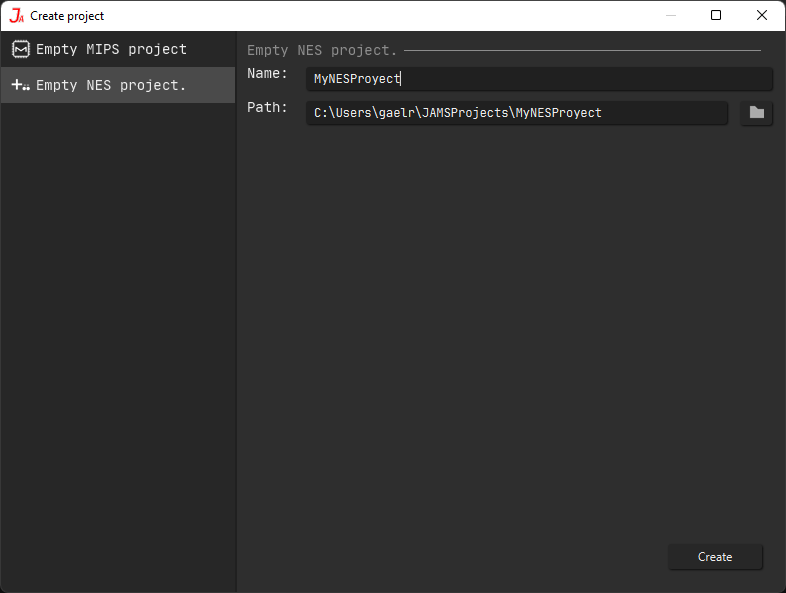
\includegraphics[width=0.8\textwidth]{images/nes/nes-project-creation}
    \caption{Creación de un proyecto \textit{NES}}
    \label{fig:nes-project-creation}
\end{figure}

\textit{NES4JAMS} añade un nuevo tipo de proyecto
que incorpora todas las herramientas para el desarrollo
de videojuegos de \textit{NES}.
Los usuarios podrán crear nuevos proyectos de este tipo
desde el menú de creación de proyectos.
Como los proyectos de \textit{NES} están destinados
a una consola muy específica, el usuario solo debe
especificar \textbf{el nombre y la localización del proyecto},
como se puede observar en la figura \ref{fig:nes-project-creation}.

Una vez creado el proyecto, \textit{JAMS} mostrará una ventana
principal muy similar a la de los proyectos \textit{MIPS32}.

\section{Editor}\label{sec:editor}

Los desarrolladores de videojuegos de \textit{NES} trabajan con
dos tipos de archivo principales: los archivos \textit{asm}
para el código y los archivos \textit{pcx} para los gráficos.
\textit{NES4JAMS} permite al usuario editar los dos tipos de archivo
de manera sencilla.

Cuando el usuario desea editar uno de estos archivos,
debe seleccionarlo en la herramienta \textbf{explorador}.
Esta herramienta muestra una representación en forma de árbol
de la estructura del proyecto.
El usuario puede expandir y contraer carpetas, así como crear,
borrar y mover archivos.
Si el usuario usa el doble clic sobre un archivo editable, este se abrirá
en el editor.
Dependiendo del tipo de archivo, el editor será diferente,
como se puede observar en la figura \ref{fig:jams-nes-editor}.

\begin{figure}[h]
    \centering
    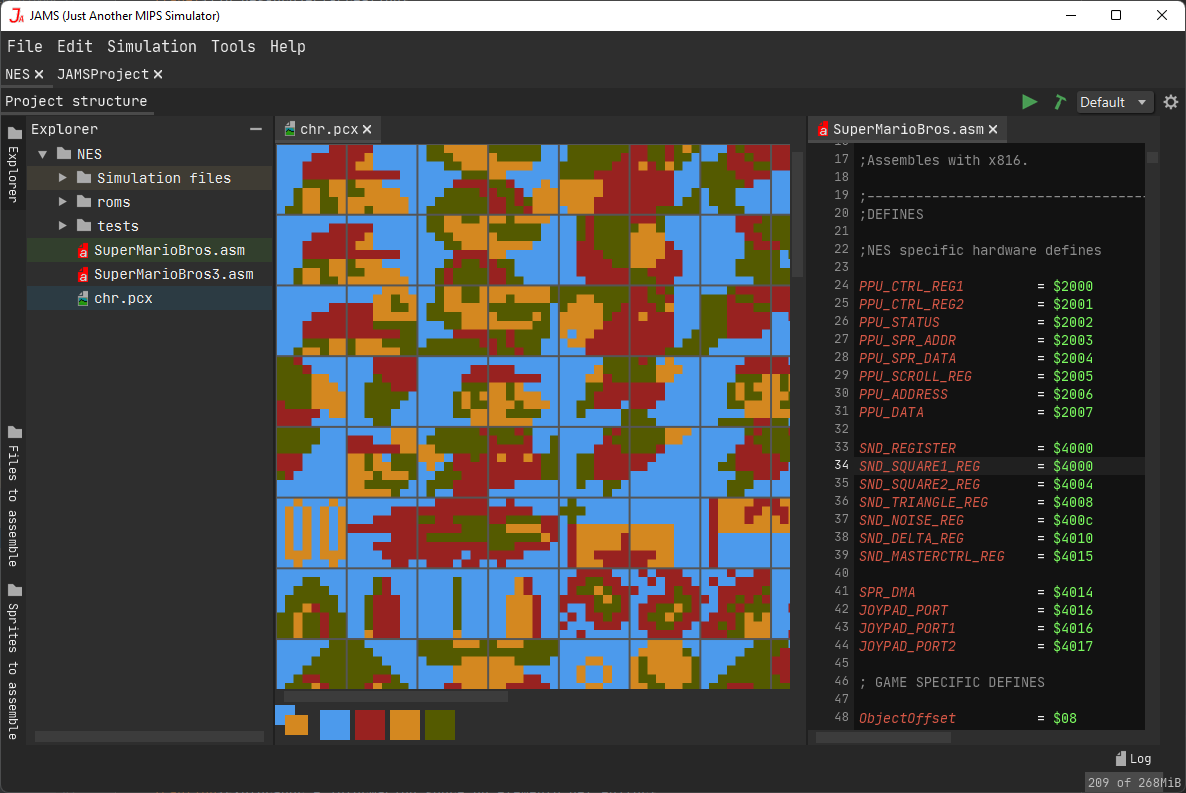
\includegraphics[width=0.8\textwidth]{images/nes/nes-editor}
    \caption{Editor de código y de gráficos junto con el explorador}
    \label{fig:jams-nes-editor}
\end{figure}

El menú contextual del explorador presenta varias acciones que
pueden ejecutarse sobre las carpetas y los archivos
del proyecto.
Una de las opciones más particulares es la opción de añadir o eliminar
archivos de código o de gráficos del ensamblador.
Al ser \textit{JAMS} un entorno de desarrollo basado en \textbf{proyectos},
se ha de proporcionar una manera de incluir o excluir archivos del
videojuego resultante.
Con este simple sistema, el usuario podrá elegir qué archivos se debe ensamblar.
Los archivos a ensamblar estarán marcados en \textbf{verde} en el explorador,
y aparecerán en orden en los nodos \textbf{Archivos a ensamblar} y
\textbf{\textit{Sprites} a ensamblar}.
Cabe destacar que, como se verá más adelante, los el orden de ensamblaje
importa, por lo que esta herramienta permite ordenarlos de una manera sencilla.

Una vez el usuario abra un archivo, su editor aparecerá en la herramienta
principal de la sección: \textbf{el visualizador de archivos}.
\textit{NES4JAMS} implementa dos editores nuevos a \textit{JAMS}:
el editor de código \textit{MOS 6502} y el editor de gráficos \textit{PCX}.

El editor de código usa el sistema de indexación desarrollado
en la capa base de \textit{JAMS}, por lo que este editor también
puede considerarse un \textbf{editor de texto inteligente}:
el editor convierte el texto puro en los componentes ensamblador
representados, pudiendo así aportar ayudas al usuario.
El editor también tiene conocimiento de las referencias y el alcance de
todas las etiquetas y macros, tanto en el propio archivo a editar
como en el resto de archivos a ensamblar.

El editor de archivos \textit{PCX} permite modificar los
gráficos del videojuego de una manera rápida y sencilla.
Este editor está pensado exclusivamente para gráficos
de \textit{NES}, por lo que cada pixel solo puede tomar
cuatro valores.
El color final se buscará en la paleta seleccionada.
El usuario puede cambiar el color de cada valor de la
paleta utilizando el botón central del ratón sobre
la casilla a cambiar.
El usuario también puede emplear el botón principal
del ratón mientras mantiene pulsada la tecla $Ctrl$.
